\section{Étape 1 : Modélisation du Problème d'Assignation}

Le travail se fera pour 4 SR et 22 territoires à attribuer pour nous verrons si notre modèle tient à l'échelle pour 10 SR et 100 zones dans l'étape 2.

\subsection{Formulation des modèles mono-objectifs}
Dans un premier temps, deux modèles mathématiques sont formulés pour résoudre le problème d'assignation des représentants de vente aux territoires. 
Le premier modèle vise à minimiser la distance totale parcourue par les représentants, tandis que le second cherche à minimiser la perturbation causée par une nouvelle répartition des zones.

Soit :
\begin{itemize}
    \item $x_{ij}$ une variable binaire indiquant si la zone $i$ est assignée au représentant $j$.
    \item $d_{ij}$ la distance entre le centre du territoire du représentant $j$ et la zone $i$.
    \item $p_i$ la charge de travail nouvelle associée au changement de l'affectation de la zone $i$.
\end{itemize}

L'objectif de minimisation de la distance est donné par :
\begin{equation}
    \min \sum_{i,j} d_{ij} x_{ij}
\end{equation}
Cet objectif permet de minimiser la distance parcourue par l'ensemble des représentants, sans prendre en compte si la distance parcourue est équilibrée.

L'objectif de minimisation de la perturbation est donné par :
\begin{equation}
    \min \sum_{i} p_i x_{ij}
\end{equation}

Nous avons de même essayé un second objectif de minimisation pour la distance :
\begin{equation}
    \min \max \sum_{i,j} d_{ij} x_{ij}
\end{equation}
Cet objectif permet de rendre la répartition plus équitable, car on minimise la distance parcourue par le représentant qui en parcourt le maximum. Chaque représentant aura alors un travail plus équitable.

Sous contraintes :
\begin{itemize}
    \item Chaque zone est assignée à exactement un représentant.
    \item La charge de travail de chaque représentant est équilibrée (c'est à dire, inférieure à 1.2 et supérieure à 0.8).
    \item Les représentants ne peuvent pas être déplacés
\end{itemize}

\subsection{Résolution avec GUROBI}
Les modèles formulés sont implémentés et résolus avec l'optimiseur GUROBI. L'instance test comprend 22 zones et 4 représentants de vente.

Les étapes de l'implémentation incluent :
\begin{itemize}
    \item Définition des variables de décision.
    \item Définition des contraintes du modèle.
    \item Résolution et analyse des solutions obtenues.
\end{itemize}

La solution pour la minimisation mono-objective de la nouvelle charge de travail (disruption) donne une valeur de 0.170.

La solution optimale du mono-objectif de minimisation de la distance totale donne une valeur de 56. 

Pour pouvoir transformer l'optimisation non linéaire du Min(Max), il suffit seulement de rajouter une variable $z$ qui est le maximum de toutes les distances parcourues par les représentants. On peut alors ajouter une contrainte pour que $z$ soit supérieur à toutes les distances parcourues par les représentants.
\subsection{Exploration des solutions non-dominées}
Une approche par contrainte-épsilon est utilisée pour générer l’ensemble des solutions non-dominées. L’idée est d’imposer des contraintes successives sur l’un des objectifs (la distance totale)  tout en minimisant l’autre (disruption).

L’analyse est réalisée avec trois niveaux de contraintes sur la charge de travail :
\begin{itemize}
    \item 1. [0.8, 1.2]
    \item 2. [0.85, 1.15]
    \item 3. [0.9, 1.1]
\end{itemize}

Chaque ensemble de solutions est visualisé à l’aide de graphes comparant la distance et la perturbation ci-dessous :

\begin{figure}[H]
    \centering
    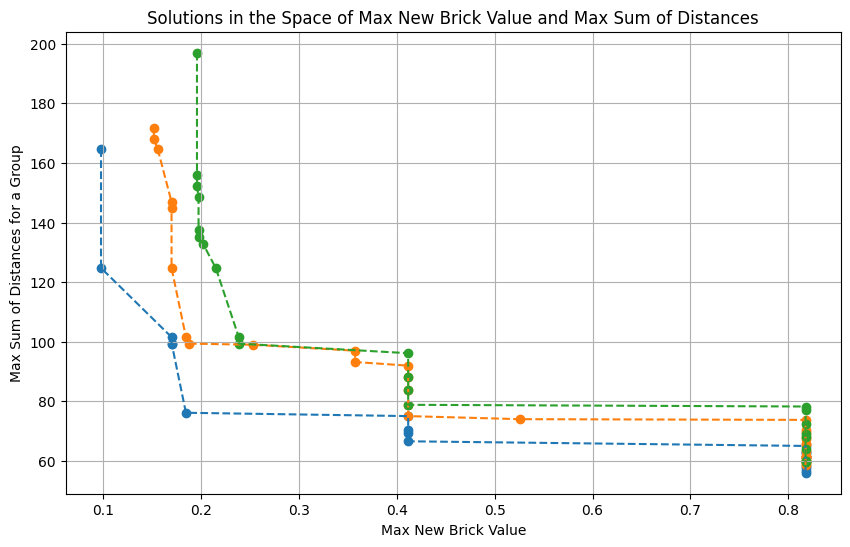
\includegraphics[width=\textwidth]{Images/step_1/step_1-min-distance.png}
    \caption{Solutions non-dominées pour des charges de travail selon 1. en bleu, 2. en orange et 3. en vert}
    \label{fig:nom_de_reference}
\end{figure}
